
%% bare_conf.tex
%% V1.4
%% 2012/12/27
%% by Michael Shell
%% See:
%% http://www.michaelshell.org/
%% for current contact information.
%%
%% This is a skeleton file demonstrating the use of IEEEtran.cls
%% (requires IEEEtran.cls version 1.8 or later) with an IEEE conference paper.
%%
%% Support sites:
%% http://www.michaelshell.org/tex/ieeetran/
%% http://www.ctan.org/tex-archive/macros/latex/contrib/IEEEtran/
%% and
%% http://www.ieee.org/

\documentclass[conference]{IEEEtran}
\usepackage{times}
\usepackage{epsfig}
\usepackage[numbers,sort&compress]{natbib}
\usepackage[protrusion=true,expansion=true]{microtype}              % Better 
\usepackage{multirow}
\usepackage{multicol}
\usepackage{rotating}
\usepackage{setspace}
%\usepackage{mdwlist}
\usepackage{comment}
\usepackage{color}                       % To highlight changes by author
\usepackage{xspace}
\usepackage{dcolumn} % used to correctly align numbers in tables
\usepackage[noorphans,font=itshape]{quoting}
\usepackage[english]{babel}

\setlength{\parindent}{2em}
\setlength{\parskip}{1em}
\renewcommand{\baselinestretch}{1.2}


%This is used with dcolumn.sty. Defines the "." to be the line up character.
\newcolumntype{.}{D{.}{.}{2}}
\newcolumntype{f}{D{.}{.}{2}}
\newcolumntype{d}{D{.}{.}{0}}
%% Example: \begin{tabular}{|l|.|.|.|.|.|.|.|.||.|.|}


% Some very useful LaTeX packages include:
% (uncomment the ones you want to load)


% *** MISC UTILITY PACKAGES ***
%
%\usepackage{ifpdf}
% Heiko Oberdiek's ifpdf.sty is very useful if you need conditional
% compilation based on whether the output is pdf or dvi.
% usage:
% \ifpdf
%   % pdf code
% \else
%   % dvi code
% \fi
% The latest version of ifpdf.sty can be obtained from:
% http://www.ctan.org/tex-archive/macros/latex/contrib/oberdiek/
% Also, note that IEEEtran.cls V1.7 and later provides a builtin
% \ifCLASSINFOpdf conditional that works the same way.
% When switching from latex to pdflatex and vice-versa, the compiler may
% have to be run twice to clear warning/error messages.






% *** CITATION PACKAGES ***
%
%\usepackage{cite}
% cite.sty was written by Donald Arseneau
% V1.6 and later of IEEEtran pre-defines the format of the cite.sty package
% \cite{} output to follow that of IEEE. Loading the cite package will
% result in citation numbers being automatically sorted and properly
% "compressed/ranged". e.g., [1], [9], [2], [7], [5], [6] without using
% cite.sty will become [1], [2], [5]--[7], [9] using cite.sty. cite.sty's
% \cite will automatically add leading space, if needed. Use cite.sty's
% noadjust option (cite.sty V3.8 and later) if you want to turn this off
% such as if a citation ever needs to be enclosed in parenthesis.
% cite.sty is already installed on most LaTeX systems. Be sure and use
% version 4.0 (2003-05-27) and later if using hyperref.sty. cite.sty does
% not currently provide for hyperlinked citations.
% The latest version can be obtained at:
% http://www.ctan.org/tex-archive/macros/latex/contrib/cite/
% The documentation is contained in the cite.sty file itself.






% *** GRAPHICS RELATED PACKAGES ***
%
\ifCLASSINFOpdf
  % \usepackage[pdftex]{graphicx}
  % declare the path(s) where your graphic files are
  % \graphicspath{{../pdf/}{../jpeg/}}
  % and their extensions so you won't have to specify these with
  % every instance of \includegraphics
  % \DeclareGraphicsExtensions{.pdf,.jpeg,.png}
\else
  % or other class option (dvipsone, dvipdf, if not using dvips). graphicx
  % will default to the driver specified in the system graphics.cfg if no
  % driver is specified.
  % \usepackage[dvips]{graphicx}
  % declare the path(s) where your graphic files are
  % \graphicspath{{../eps/}}
  % and their extensions so you won't have to specify these with
  % every instance of \includegraphics
  % \DeclareGraphicsExtensions{.eps}
\fi
% graphicx was written by David Carlisle and Sebastian Rahtz. It is
% required if you want graphics, photos, etc. graphicx.sty is already
% installed on most LaTeX systems. The latest version and documentation
% can be obtained at: 
% http://www.ctan.org/tex-archive/macros/latex/required/graphics/
% Another good source of documentation is "Using Imported Graphics in
% LaTeX2e" by Keith Reckdahl which can be found at:
% http://www.ctan.org/tex-archive/info/epslatex/
%
% latex, and pdflatex in dvi mode, support graphics in encapsulated
% postscript (.eps) format. pdflatex in pdf mode supports graphics
% in .pdf, .jpeg, .png and .mps (metapost) formats. Users should ensure
% that all non-photo figures use a vector format (.eps, .pdf, .mps) and
% not a bitmapped formats (.jpeg, .png). IEEE frowns on bitmapped formats
% which can result in "jaggedy"/blurry rendering of lines and letters as
% well as large increases in file sizes.
%
% You can find documentation about the pdfTeX application at:
% http://www.tug.org/applications/pdftex





% *** MATH PACKAGES ***
%
%\usepackage[cmex10]{amsmath}
% A popular package from the American Mathematical Society that provides
% many useful and powerful commands for dealing with mathematics. If using
% it, be sure to load this package with the cmex10 option to ensure that
% only type 1 fonts will utilized at all point sizes. Without this option,
% it is possible that some math symbols, particularly those within
% footnotes, will be rendered in bitmap form which will result in a
% document that can not be IEEE Xplore compliant!
%
% Also, note that the amsmath package sets \interdisplaylinepenalty to 10000
% thus preventing page breaks from occurring within multiline equations. Use:
%\interdisplaylinepenalty=2500
% after loading amsmath to restore such page breaks as IEEEtran.cls normally
% does. amsmath.sty is already installed on most LaTeX systems. The latest
% version and documentation can be obtained at:
% http://www.ctan.org/tex-archive/macros/latex/required/amslatex/math/





% *** SPECIALIZED LIST PACKAGES ***
%
%\usepackage{algorithmic}
% algorithmic.sty was written by Peter Williams and Rogerio Brito.
% This package provides an algorithmic environment fo describing algorithms.
% You can use the algorithmic environment in-text or within a figure
% environment to provide for a floating algorithm. Do NOT use the algorithm
% floating environment provided by algorithm.sty (by the same authors) or
% algorithm2e.sty (by Christophe Fiorio) as IEEE does not use dedicated
% algorithm float types and packages that provide these will not provide
% correct IEEE style captions. The latest version and documentation of
% algorithmic.sty can be obtained at:
% http://www.ctan.org/tex-archive/macros/latex/contrib/algorithms/
% There is also a support site at:
% http://algorithms.berlios.de/index.html
% Also of interest may be the (relatively newer and more customizable)
% algorithmicx.sty package by Szasz Janos:
% http://www.ctan.org/tex-archive/macros/latex/contrib/algorithmicx/




% *** ALIGNMENT PACKAGES ***
%
%\usepackage{array}
% Frank Mittelbach's and David Carlisle's array.sty patches and improves
% the standard LaTeX2e array and tabular environments to provide better
% appearance and additional user controls. As the default LaTeX2e table
% generation code is lacking to the point of almost being broken with
% respect to the quality of the end results, all users are strongly
% advised to use an enhanced (at the very least that provided by array.sty)
% set of table tools. array.sty is already installed on most systems. The
% latest version and documentation can be obtained at:
% http://www.ctan.org/tex-archive/macros/latex/required/tools/


% IEEEtran contains the IEEEeqnarray family of commands that can be used to
% generate multiline equations as well as matrices, tables, etc., of high
% quality.




% *** SUBFIGURE PACKAGES ***
%\ifCLASSOPTIONcompsoc
%  \usepackage[caption=false,font=normalsize,labelfont=sf,textfont=sf]{subfig}
%\else
%  \usepackage[caption=false,font=footnotesize]{subfig}
%\fi
% subfig.sty, written by Steven Douglas Cochran, is the modern replacement
% for subfigure.sty, the latter of which is no longer maintained and is
% incompatible with some LaTeX packages including fixltx2e. However,
% subfig.sty requires and automatically loads Axel Sommerfeldt's caption.sty
% which will override IEEEtran.cls' handling of captions and this will result
% in non-IEEE style figure/table captions. To prevent this problem, be sure
% and invoke subfig.sty's "caption=false" package option (available since
% subfig.sty version 1.3, 2005/06/28) as this is will preserve IEEEtran.cls
% handling of captions.
% Note that the Computer Society format requires a larger sans serif font
% than the serif footnote size font used in traditional IEEE formatting
% and thus the need to invoke different subfig.sty package options depending
% on whether compsoc mode has been enabled.
%
% The latest version and documentation of subfig.sty can be obtained at:
% http://www.ctan.org/tex-archive/macros/latex/contrib/subfig/




% *** FLOAT PACKAGES ***
%
%\usepackage{fixltx2e}
% fixltx2e, the successor to the earlier fix2col.sty, was written by
% Frank Mittelbach and David Carlisle. This package corrects a few problems
% in the LaTeX2e kernel, the most notable of which is that in current
% LaTeX2e releases, the ordering of single and double column floats is not
% guaranteed to be preserved. Thus, an unpatched LaTeX2e can allow a
% single column figure to be placed prior to an earlier double column
% figure. The latest version and documentation can be found at:
% http://www.ctan.org/tex-archive/macros/latex/base/


%\usepackage{stfloats}
% stfloats.sty was written by Sigitas Tolusis. This package gives LaTeX2e
% the ability to do double column floats at the bottom of the page as well
% as the top. (e.g., "\begin{figure*}[!b]" is not normally possible in
% LaTeX2e). It also provides a command:
%\fnbelowfloat
% to enable the placement of footnotes below bottom floats (the standard
% LaTeX2e kernel puts them above bottom floats). This is an invasive package
% which rewrites many portions of the LaTeX2e float routines. It may not work
% with other packages that modify the LaTeX2e float routines. The latest
% version and documentation can be obtained at:
% http://www.ctan.org/tex-archive/macros/latex/contrib/sttools/
% Do not use the stfloats baselinefloat ability as IEEE does not allow
% \baselineskip to stretch. Authors submitting work to the IEEE should note
% that IEEE rarely uses double column equations and that authors should try
% to avoid such use. Do not be tempted to use the cuted.sty or midfloat.sty
% packages (also by Sigitas Tolusis) as IEEE does not format its papers in
% such ways.
% Do not attempt to use stfloats with fixltx2e as they are incompatible.
% Instead, use Morten Hogholm'a dblfloatfix which combines the features
% of both fixltx2e and stfloats:
%
% \usepackage{dblfloatfix}
% The latest version can be found at:
% http://www.ctan.org/tex-archive/macros/latex/contrib/dblfloatfix/




% *** PDF, URL AND HYPERLINK PACKAGES ***
%
%\usepackage{url}
% url.sty was written by Donald Arseneau. It provides better support for
% handling and breaking URLs. url.sty is already installed on most LaTeX
% systems. The latest version and documentation can be obtained at:
% http://www.ctan.org/tex-archive/macros/latex/contrib/url/
% Basically, \url{my_url_here}.




% *** Do not adjust lengths that control margins, column widths, etc. ***
% *** Do not use packages that alter fonts (such as pslatex).         ***
% There should be no need to do such things with IEEEtran.cls V1.6 and later.
% (Unless specifically asked to do so by the journal or conference you plan
% to submit to, of course. )


% correct bad hyphenation here
\hyphenation{op-tical net-works semi-conduc-tor}


\begin{document}
%
% paper title
% can use linebreaks \\ within to get better formatting as desired
% Do not put math or special symbols in the title.
\title{Running Head}


% author names and affiliations
% use a multiple column layout for up to three different
% affiliations
\author{\IEEEauthorblockN{Anthony Escalona}
\IEEEauthorblockA{
	Seidenberg School of CSIS \\
	New York, Ny 10038 \\
	Email: ae50483p@pace.edu
	}
}



% make the title area
\maketitle{}

% As a general rule, do not put math, special symbols or citations
% in the abstract
\begin{abstract}
Roadway traffic safety is a significant concern for transportation governing agencies as well as ordinary citizens.  To provide advice for safe driving, careful analysis of road traffic information is important to identify variables closely related to fatal accidents.  In this paper, I apply statistical analysis and data mining algorithms on the NYC Open Data portal dataset as an attempt to address these problems. The relationship between fatal rate and other attributes, including collision manner, weather, surface condition, and light condition, were investigated.
\end{abstract}

\section{Introduction}
\label{sec:introduction}

It is estimated that around 4,000 New Yorkers are seriously injured in New York and more than 250 people are killed in traffic accidents every year. The automobile is the leading cause of injury-related death for children under 14 years of age and the second leading cause for seniors. On average, every two hours, vehicles severely injure or kill a New Yorker. The cost of these deaths and injuries impacts the city's social and economic growth greatly.  New York City should no longer consider traffic crashes as mere "accidents," but as preventable incidents that can be addressed systematically. No degree of fatality is unavoidable or appropriate on the streets of the city. New York City's Vision Zero Action Plan\cite{VisionZero} is the foundation to reduce traffic deaths and injuries. City of New York will use every available tool to enhance the safety of our streets. With this action plan, it is making a bold new commitment to improving street safety in every neighborhood and district – with increased enforcement of dangerous moving violations such as speed and failure to yield to pedestrians, new street designs and configurations to improve safety, widespread public access and communications, and a comprehensive legislative agenda to increase penalties. 

Data mining is a major step in knowledge discovery.  It is the process of extraction of non-trivial, valid and potentially useful information from huge databases. Some of the important data mining techniques are classification, association rule mining, segmentation, and clustering. 

Predicting where and when road incidents will occur is complicated. It is possible to analyze traffic injury statistics and identify a correlation between variables based on historical traffic event data. On the other hand, visualization of data from traffic accidents provides detailed insights into how it changes over time. This paper focuses on practical issues related to the project to prevent road accidents. Analysis and visualization of data help observe the occurrence of traffic accidents and take appropriate action to enhance safety.  More interestingly, does climate lead to motor vehicle collisions? 

The paper is as follows. Section II addresses motivation. Section III addresses related work. Section IV presents data analysis and evaluation lessons learned. Section V concludes and outlines future work. 

\section{Motivation}
NYC’s Vision Zero Action Plan was launched in 2014, detailing 63 different programs that are implemented by the Mayor's Office and several City Agencies to minimize mortality and serious injury. The Vision Zero Task Force has since launched 143 new initiatives for a total of 206 initiatives (40 new initiatives were implemented in 2015, 22 were added in 2016, 26 in 2017, 27 in 2018 and 28 in 2019).  City Agencies separate these programs and continue to make progress on their following measures \cite{VisionZeroInitiative}:     

\begin{enumerate}  
	\item New York City Department of Transportation (DOT):
	\begin{enumerate}
		\item Launch an integrated speed reducer installation program
		\item Install speed cameras at additional school zone locations
		\item Expand and enhance People Priority Streets to improve pedestrian safety and access
	\end{enumerate}  
	\item New York Police Department (NYPD):
	\begin{enumerate}
		\item Expand outreach and enforcement regarding the safe execution of left and right hand turns by all motorists
		\item Expand NYPD's clear bus routes enforcement action plan
		\item Increase safety within the trade waste and private carting industry through outreach and enforcement   
	\end{enumerate}
	\item New York City Taxi \& Limousine Commission (TLC):
	\begin{enumerate}
		\item Ensure TLC-licensed vehicles with outstanding part recalls are fixed in a timely manner
		\item Reduce use of left turns
		\item Introduce predictive analytics relating to driving behaviors and crashes through CRASHStat and the Fleet Office of Real Time Tracking (FORT)
	\end{enumerate}
\end{enumerate}

More vigorous enforcement of dangerous driving behavior by the NYPD and the TLC may help to reduce traffic fatalities and serious injuries. In addition to greater enforcement, efforts are being made to upgrade equipment and technology for speed detection, increase the number of staff on the highway unit, and expand the breadth of information and data captured to preserve crash details better. Finally, the purpose of the data analysis is to derive useful data from the data source and to further use it for visualization by using statistical models.     
\section{Literature Review}
A number of studies have been conducted to determine the factors leading to serious road accidents and to reduce the number and severity of injuries by removing or regulating these factors. As the traffic accident is large and heterogeneous, most scientists adopted data mining methods to carry out their studies.

Chong, Abraham, and Paprzycki \cite{chong2004traffic} have applied artificial neural networks and decision trees to a specific data collection from the National Automotive Sampling Program and General Estimates Systems including traffic incident information from 1995 to 2000. The collection of data was limited only to head-on collisions. The findings revealed that neural networks were outperformed by the decision tree approach. The findings found that seat belt use, highway lighting condition, and driver alcohol use were the most important variables in fatal injuries.

Authors in \cite{Bedard} have applied their work using multivariate logistic regression to determine the independent contribution of driver, crash, and vehicle characteristics to driver' fatality. The result showed that increased use of seatbelts, reduced vehicle speed, and reduced number of and severity of drivers' side-impact might prevent deaths.

The purpose of paper \cite{SingletonFactors} was to employ logistic regression models to develop crash-related injury prediction models. They analyzed traffic crash data in Kentucky during 2001 using logistic regressions. They concluded that the occupant’s risk factors for the high level of injury severity were age, gender, and non-use of restraints. In \cite{ associationHanrahan}, the authors used the same model to quantify the association of driver’s age with traffic injury severity. Wisconsin crash data from 2000 to 2004 was used to study 602,694 drivers of a car or truck who were involved in a motor vehicle crash. It was discovered that the oldest drivers, especially those older than 85 drivers 85 years and older, had the highest risks for serious injury or fatality.


\section{Data Analysis and Evaluation}
\subsection{Background}
The following information should provide enough background for the reader unfamiliar with Logistic Regression to understand the points made in this paper. Readers already familiar with Logistic Regression can skip to the next section. It is a statistical method used to evaluate a dataset in which one or more independent variables calculate an outcome. The result is measured by a dichotomous variable in which there are only two possible outcomes. It uses a formula, like linear regression, as the representation. However, the outcome variable is categorical like two-valued outcomes like true/false, pass/fail, or yes/no. To predict value y, input values x are combined linearly using weights or coefficient values as beta. A key difference from linear regression is that the computation output value is a binary number (0 or 1) instead of a numerical value.  Below is an example logistic regression equation:
 
y = e\^ (b0 + b1*x) / (1 + e\^(b0 + b1*x))
\newline 
\newline
Where y is the predicted output, b0 is the bias or intercept term, and b1 is the coefficient for the single input value x. Each column in the input data has an associated b coefficient, a constant real value, that must be learned from data.
%https://machinelearningmastery.com/logistic-regression-for-machine-learning/

\subsection{Methodology}
%https://www.reddit.com/r/learnpython/comments/41s9q5/classifying_latitude_and_longitude_into_suburbs/
To visualize data, I used the Python programming language.  All necessary libraries loaded, and the script required the following libraries: 1) google.cloud to access BigQuery database, 2) pandas for data frame management, 3) Matplot for visuals, and 4) Numpy to perform scientific computing.  For making requests, Google authentication is mandatory. The python code must set the google\_application\_credentials environment variable. Replace [PATH] with the JSON file path that contains the service account key and the filename of [FILE NAME]. The attribute is for the current shell session only.

The collision data are made available through the NYC Open Data initiative and can also be searched through the BigQuery Community Datasets offered by Google. For comparison with collision data, historical weather data from NOAA weather data were used.  Google BigQuery makes both NOAA weather data and NYPD traffic collisions available publicly. The first phase was the compilation of daily NYC weather data using years from 2012 to 2019 and limit the return query to the New York City Area. 
\begin{figure}[bth]
	\centering
	\scalebox{1}{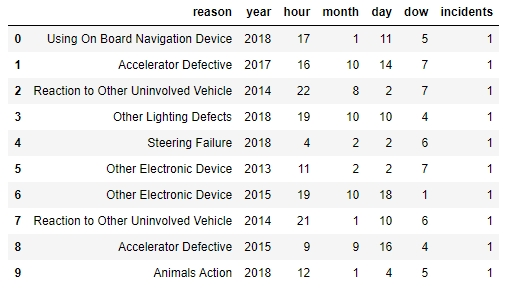
\includegraphics{../figures/mvtable.jpg}}
	\caption{NYC Motor Vehicle Collisions Crash Table}
	\label{fig:mvtable}
\end{figure}
\begin{figure}[bth]
	\centering
	\scalebox{1}{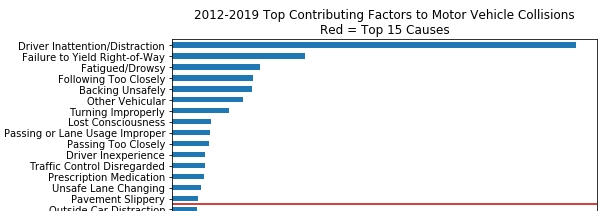
\includegraphics{../figures/crashPlot.jpg}}
	\caption{Contributing Factors}
	\label{fig:crashPlot}
\end{figure}
The first table (fig \ref{fig:mvtable}) of data contains the number of motor vehicle collisions reported per year, month, day, and day of the week (dow). This ranges from 2012 to 2019 and has nearly 30 forms of explanations along with the associated counts of the incidents.  As a crash data baseline, figure \ref{fig:crashPlot} plots the top contributing factors for collisions. According to the data, the leading cause of crashes is distraction. 
\newline \newline
Next, the second table of data contains weather data reported by element, year, month, day, dow, and location name (fig \ref{fig:noaatable}).
\begin{figure}[bth]
	\centering
	\scalebox{1}{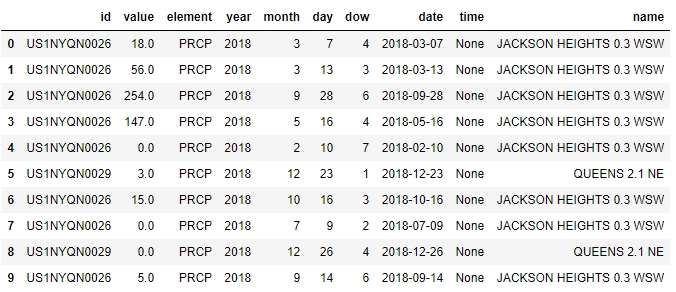
\includegraphics{../figures/noaatable.jpg}}
	\caption{NOAA Weather Table}
	\label{fig:noaatable}
\end{figure}
\newline 
The correlation matrix was used to estimate the linear historical relationship between the returns of the weather variables. IsWeekend (Sat, Sun) feature was added instead of dow. The built-in .corr() method on a pandas DataFrame calculated the correlation matrix. Correlation ranges from -1 to 1. The matrix shows correlation coefficients between weather, x-axis, and contributing factor. Each cell in the table shows the correlation between the two variables (fig \ref{fig:cormap}). 

\begin{figure}[bth]
	\centering
	\scalebox{1}{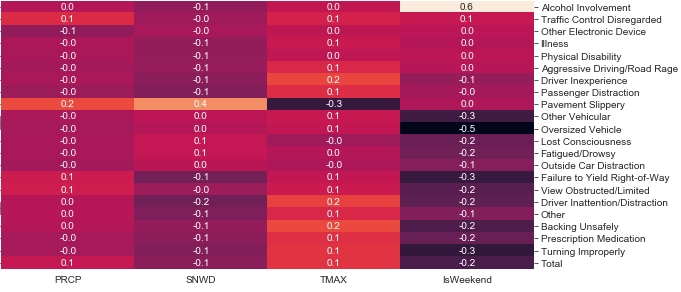
\includegraphics{../figures/cormap.jpg}}
	\caption{Correlation Matrix}
	\label{fig:cormap}
\end{figure}

\subsection{Observations}
Based on observations, There are some interesting patterns to see. Alcohol accidents are correlated with the weekend. Illness, physical disability, and road rage seem to occur regardless of weather patterns, maybe slightly influenced by temperature. Driver distraction, passenger distraction, and inexperience are correlated with higher temperatures. The other type of road traffic accidents was drop out of analysis due to the low number of occurrences. Visualization and data analysis of road traffic. 
\section{Conclusion and Future Work}
The conclusion goes here.
 



% conference papers do not normally have an appendix


% use section* for acknowledgement
\section*{Acknowledgment}
The authors would like to thank...


\bibliographystyle{IEEEtran}
{\small\bibliography{references}}
 

\end{document}


